\ifx\wholebook\relax\else
\input{../Common.tex}
\input{../macroes.tex}
\begin{document}
\fi

\chapter{Conditions}\label{cha:condition}\label{cha:conditional}

Up until now the programs you defined executed \textit{all} the expressions they contained, them one after the other. You had no way to say that certain messages should only be executed when certain \textit{conditions were met}. This chapter and the next one introduce an important programming concept: the notion of \emph{conditional} \index{condition} execution, \ie\ the fact that a certain piece of code executes only when a specified condition holds. A condition is an expression that can be true or false. 

This chapter starts with defining a simple problem that shows the need for conditional execution.  Then it presents that a conditional expression is composed of a\emph{ condition} and a \emph{conditional block} --- that is a sequence of expressions that are conditionally executed.

\section{A Simple Problem}

Suppose you want to change the color of a robot depending on its distance from the center of the screen. If a robot is less than 200 pixels from the center, it should be red otherwise it should be green. This problem requires a \textit{conditional} execution. Depending on a condition --- the robot's location --- its color should change. 

The method \ct{distanceDetector} shows a possible solution, and \scrref{scr:detector} shows how the method \ct{distanceDetector} is used. 

\begin{scriptwithtitle}{A Simple Detector}\label{scr:detector}
\caro := \Turtle new.
\caro jump: 20.
\caro distanceDetector.
\caro jump: 200.
\caro distanceDetector.
\end{scriptwithtitle}

\begin{method}\label{mth:detector}
\textbf{distanceDetector}

   | distanceFromCenter | 
   distanceFromCenter := self distanceFrom: World center.
   distanceFromCenter < 200
      ifTrue: [ self color: Color red ]
      ifFalse: [ self color: Color green ]
\end{method}

Let's analyze what happens when the expression \ct{\caro distanceDetector} is executed. 

\begin{enumerate}
\item The expression \ct{self distanceFrom: World center} computes the distance from the receiver to the center of the screen. This distance is stored into the variable \ct{distanceFromCenter}. 

\item Then the expression \ct{distanceFromCenter < 200 ifTrue: [ self color: Color red ] ifFalse: [ self color: Color green ]} is executed as follows: \textit{if} the distance is smaller than 200 the color of the receiver is changed to re; otherwise it is changed to green. This expression is a \textit{conditional} expression. It is spread over three lines in the method definition but it is all one expression, because there is no period to terminate it earlier.
\end{enumerate}

\begin{figure}[h]
\begin{center}
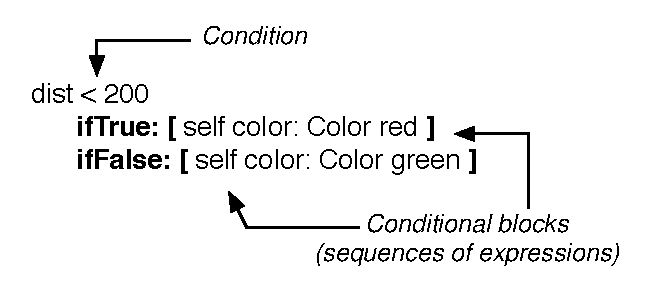
\includegraphics{distanceDetector}
\caption{A conditional expression is composed of a condition and conditional block (a conditional sequence of expressions).\label{fig:distanceDetector}}
\end{center}
\end{figure}

A conditional expression is composed of two parts: a \index{condition}\textit{condition} and \index{conditional block} \textit{conditional block} that is a sequence of expressions. 
The expression \ct{distanceFromCenter < 200} is a condition and the expressions \ct{[self color: Color red]} and \ct{[self color: Color green]} are conditional blocks  as shown by Figure~\ref{fig:distanceDetector}. 

The method \ct{ifTrue:ifFalse:} executes one condition, here \ct{distanceFromCenter < 200}, and depending of its value, executes one of the conditional blocks and skip the other. The keyword \ct{ifTrue:} indicates that the conditional block \ct{[ self color: Color red ]} is only executed when the condition is true. Similarly the keyword \ct{ifFalse:} indicates that  the conditional block  \ct{[ self color: Color green ]} is only executed when the condition is false. The conditional blocks are also called the condition \emph{branches}.  Imagine that you would follow the trunk of a tree with your finger, each time you encounter a branch you would have to choose which path you want to follow, and you would follow only one at a time. The term branch refers to this situation. It represents the fact that the execution will have to choose between branches and only execute one at a time.


So there are different kinds of expressions. Some such as \ct{self distanceFrom: World center} are always executed while others are executed only when their associated condition holds. 

 A condition is not limited to one single expression but can contain a composition of expression as I will present in Chapter~\ref{cha:boolean}. The method \ct{ifTrue:ifFalse:} defines two possible blocks, which can each contain a sequence of expressions.  Note that the method \ct{ifTrue:ifFalse:} is a \textit{single} method with two arguments, one for the true case and one for the false case. Therefore you should not put a period after the \ct{]} following the \ct{ifTrue:} as it will break the conditional statement by ending it too soon, causing an error.

\paragraph{Adding a Trace to Understand.} To understand how conditional expressions are executed, I suggest you use the Transcript and send it messages to generate trace  as presented in Chapter~\ref{ch:strings}. You can also use the debugger by inserting the expression \ct{self halt} as shown in the Chapter~\ref{ch:debugger}. If you want to know whether a particular  branch is executed, introduce expressions such as \ct{Transcript show: 'here' ; cr} in the branch.  Method~\ref{mth:detectorTrans} presents one way to generate such a trace in the context of the \ct{distanceDetector} method. Depending on the position of the robot different traces will be produced. Try to guess them before executing script~\ref{scr:detector}. Do not hesitate to add and modify such a trace in all the scripts you have problem to understand. 

\begin{method}\label{mth:detectorTrans}
\textbf{distanceDetector}

   | distanceFromCenter | 
   distanceFromCenter := self distanceFrom: World center.
   \textbf{Transcript show: 'always'; cr.}
   distanceFromCenter < 200
      ifTrue: [ self color: Color red.
              \textbf{Transcript show: 'red' ; cr ]}
      ifFalse: [ self color: Color green
               \textbf{Transcript show: 'green' ; cr ]}
\end{method}


%\paragraph{\ct{ifTrue:ifFalse} and \ct{ifFalse:ifTrue:}.}
%The method \ct{ifFalse:ifTrue:} also exists. It works the same way the method \ct{ifTrue:ifFalse:}, \ie it executes the false case when the condition is false and the true one when the condition is true, exactly as the method \ct{ifTrue:ifFalse:}. This method is just to help you write more readable code if you want to start with the messages executed when the condition is false as shown by Figure~\ref{fig:conditionalifTifFifFifT}.

%
%\begin{figure}[h]
%\begin{center}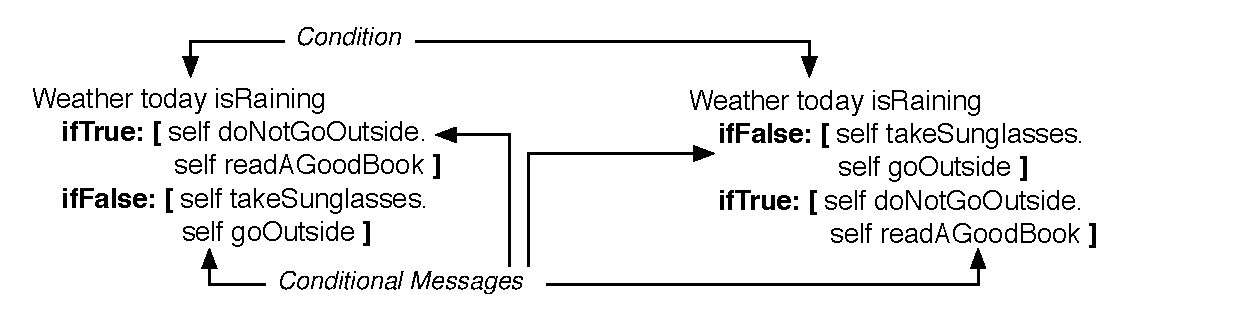
\includegraphics[width=\linewidth]{conditionalifTifFifFifT}
%\caption{Two equivalent conditionals expressions.\label{fig:conditionalifTifFifFifT}}\end{center}
%\end{figure}


\paragraph{About the Value Returned by a Method.}
When I presented how to define methods in Chapter~\ref{ch:turtleTeaching} I explained that executing a method not only evaluates the messages it contains but also \emph{returns} a value.  Up until now you did not really used the result returned by methods. Now for the condition expression we are essentially interested by the result returned by the method. For example in method \ref{mth:detector}, the expression  \ct{self distanceFrom: World center} not only computes the distance of the receiver from the center of the screen but \textit{returns} it.  The condition expression, \ct{distanceFromCenter < 200}, uses this value to decide wich branch should be executed. Note that the expression \ct{distanceFromCenter < 200} also returns a value telling whether the distance is smaller or not than 200 (see Chapter~\ref{cha:boolean}). 

\fprod{production the following should be in a frame}
A conditional expression is composed of two parts: a \index{condition}\textit{condition} and \index{conditional messages} \textit{conditional messages}. 

\begin{nalltt}
\textit{aCondition}
\quad  \textbf{ifTrue: [} \textit{expressionsIfConditionIsTrue}\textbf{]}
\quad  \textbf{ifFalse: [} \textit{expressionsIfConditionIsFalse} \textbf{]}
\end{nalltt}

%\textit{aCondition}
%\quad   \textbf{ifFalse: [} \textit{messagesIfConditionIsFalse} \textbf{]}
%\quad   \textbf{ifTrue: [} \textit{messagesIfConditionIsTrue} \textbf{]} 

\fprod{until here}

\section{Two Other Conditional Messages: \ct{ifTrue:} and \ct{ifFalse:}}

Sometimes you only need to perform one action when a specific condition is true but do nothing when the condition is false (or vice versa). For example the method \ct{redWhenCloseToCenter} (\ref{mth:redWhenCloseToCenter}) only changes the color of the receiver to red when it is at a distance smaller than 200 pixels from the screen center. 

\begin{method}\label{mth:redWhenCloseToCenter}
\textbf{redWhenCloseToCenter}

   | distanceFromCenter | 
   distanceFromCenter := self distanceFrom: World center.
   distanceFromCenter < 200
      \bold{ifTrue: [} self color: Color red \bold{]}
      \bold{ifFalse: [ ]}
\end{method}

Using the method \ct{ifTrue:ifFalse:} you just have to leave the second branch empty \ie\ \ct{[ ]}. However, \st provides two other methods \ct{ifTrue:} and \ct{ifFalse:} to express these kinds of conditional expressions. The method \ct{ifTrue:} executes its conditional block when its condition is true. Using the method \ct{ifTrue:} I rewrite the method \ct{redWhenCloseToCenter} shown in \ref{mth:redWhenCloseToCenter} as shown in \mthref{mth:redWhenCloseToCenter2}.

\begin{method}\label{mth:redWhenCloseToCenter2}
\textbf{redWhenCloseToCenter}

   | distanceFromCenter | 
   distanceFromCenter := self distanceFrom: World  center.
   distanceFromCenter < 200
      \bold{ifTrue:} [ self color: Color red ]
\end{method}

Contrary to \ct{ifTrue:}, the method \ct{ifFalse:} executes its conditional block when its condition is \emph{false}. The methods \ct{ifFalse:} and \ct{ifFalse:} both execute a condition and, depending on the value returned by the condition, either execute or skip the conditional block. 

%Note that you can always negate (logically reverse) a condition to switch from one form to the other. For example in method~\ref{mth:redWhenCloseToCenter3}, \ct{distanceFromCenter >= 200} is the negation of the expression \ct{distanceFromCenter < 200}. Again I suggest you add a trace to understand what is happening.

%
%\begin{method}\label{mth:redWhenCloseToCenter3}
%redWhenCloseToCenter

%   | distanceFromCenter | 
%   distanceFromCenter := self distanceFrom: World  center.
%   \bold{distanceFromCenter >= 200}
%      \bold{ifFalse:} [ self color: Color red ]
%\end{method}


\fprod{production the following should be in a frame}
The method \ct{ifTrue:} executes its conditional block when its condition is true.
The method \ct{ifFalse:} executes its conditional block when its condition is false.

\begin{nalltt}
\textit{aCondition}
      \textbf{ifTrue: [} \textit{expressionsIfConditionIsTrue} \textbf{]}

\textit{aCondition}
      \textbf{ifFalse: [} \textit{expressionsIfConditionIsFalse} \textbf{]}
\end{nalltt}
\fprod{until here}

\paragraph{A Subtle Point.} The difference between using \ct{ifTrue:ifFalse:}, and \ct{ifTrue:} followed by \ct{ifFalse:} is that the \textit{condition} using \ct{ifTrue:ifFalse:} is only executed once, while with \ct{ifTrue:} followed by \ct{ifFalse:} the conditions of the \emph{two} conditional expressions are executed. This can be a problem when the conditional block of the first conditional expression (\ct{ifTrue:}) modify what is tested by the condition of the second conditional expression (\ct{ifFalse:}). In such a case using \ct{ifTrue:} followed by \ct{ifFalse:} is not equivalent to using \ct{ifTrue:ifFalse:}.


\section{Nesting Conditional Expressions}
A conditional expression can contain any other expressions and in particular other conditional expressions. This is what I demonstrate next. There is nothing spectacular about it, but it is common --- and that is why I want to show it to you. Conditions can be nested inside conditions.

\paragraph{Another Simple Problem.}
Let's modify the previous problem. Now if a robot is less than 200 pixels from the center it should be red; when it is between 200 and 300 pixels away, it should be yellow; and at a distance greater than 300 it should be green.  %Figure~\ref{fig:detector} shows various robots that set their color using the method \ct{setThreeColor}. 

%\begin{figure}
%\begin{center}
%\includegraphics[width=10cm]{detector}
%\caption{Various robots at different distances from a point. \label{fig:detector}}
%\end{center}
%\end{figure}

In this problem, different parts of the method should be executed under different circumstances. The color should change to yellow  under different conditions that are different than changing the color to green. A possible solution to our problem is shown by method \ref{mth:threeColorDetector}. 

\begin{method}\label{mth:threeColorDetector}
\textbf{setThreeColor}

   | distance | 
   distance := self distanceFrom: World  center.
   distance > 300
      ifTrue: [ self color: Color green ]
      ifFalse: [ distance < 200
         ifTrue: [ self color: Color red ]
         ifFalse: [ self color: Color yellow ] ]
\end{method}

\Mthref{mth:detector4} contains the exact same code with highlighting added to show the conditional expressions. There are two different conditional expressions. The first one is shown in italics and the second in bold as shown in \tmthref{mth:detector4}. The second conditional expression (in bold) is only executed when the condition of the first conditional expression is false. When the distance is smaller than 300 the conditional expression 2 is executed. That means that its condition is executed and, depending on its values the correct branch is executed. 


\noindent
\begin{minipage}[l]{8cm}
\begin{method}\label{mth:detector4}
\textbf{setThreeColor}

   | distance | 
   distance := self distanceFrom: World  center.
   \textit{distance > 300
      ifTrue: [ self color: Color green ]
      ifFalse: [ }\textbf{distance < 200
         ifTrue: [ self color: Color red ]
         ifFalse: [ self color: Color yellow ]}\textit{]}
\end{method}
\end{minipage}
\hspace{1cm}
\begin{minipage}[r]{8cm}
\begin{nalltt}
\textrm{Condition 1:}
\textit{distance > 300
      ifTrue: [ self color: Color green ]
      ifFalse: [ ... ]}

\textrm{Condition 2:}
\textbf{distance < 200
         ifTrue: [ self color: Color red ]
         ifFalse: [ self color: Color yellow ]}
\end{nalltt}
\end{minipage}

If you have trouble to identify this two conditional expressions, pick some   particular values for the distance (like 150, 250 or 350). Take a colored pen and underline the part of each method that will be executed.  Following each step carefully will show  that only certain branches are executed. I suggest you introduce different traces to understand how the conditions are executed or using the debugger stepping slowly into the method. 

%%%%%%%%%%%%%%%%%%%%%%%%%%%%%%%%%%%%%%%%%%%%%%%%%%%%%%%%%%%%%
\section{Learning from Errors}
As people are always making mistakes, looking at errors is an excellent way to learn and understand a concept from another perspective.  I defined the method \ct{coloredTurn: anAngle} that changes the color of a robot according to the direction it is heading.   When the robot points to the north it should turn blue to represent cold. it should turn red when it points to the south, and otherwise it should be green. Our first try at defining of this method is shown in~\mthref{mth:colored}. 


\begin{method}\label{mth:colored}
\textbf{coloredTurn: anAngle}
     "change the color of the robot so that it is blue aiming 
     at the north and red to the south"

     self turn: anAngle.
     self direction = 90
         ifTrue: [ self color: Color blue ].
     self direction = -90
         ifTrue: [ self color: Color red ]
         ifFalse: [ self color: Color green ]
\end{method}

The above definition is not correct. Try to understand why before reading any farther. 
The above method is wrong because when the robot is pointing to the north, and its color is green. But it should be blue, as shown in \tscrref{scr:illustbug}.  

\begin{scriptwithtitle}{Illustrating the bug}\label{scr:illustbug} 
| \caro |
\caro := \Turtle new.
\caro coloredTurn: -90.
\caro color \pr  Color red           "ok"
\caro coloredTurn: 90.
\caro color \pr Color green.      "ok"
\caro coloredTurn: 90.
\caro color \pr Color green      "wrong"
\end{scriptwithtitle}


\paragraph{Why...} Execute~\tmthref{mth:colored} mentally to identify why this method is wrong. The problem is that even if the condition  \ct{self direction = 90} is true and its associated block is executed, the method continues and evaluates the false conditional block of the last conditional expression, changing the color of the robot to green. 
The following commented version of the code illustrates this.


\begin{nalltt}
\caro coloredTurn: 90.

   self direction = 90                                        \textrm{"is true"}
       ifTrue: [ self color: Color blue ]                 \textrm{"so the true conditional message is executed"}        
                                                                             \textrm{"the robot becomes blue and evaluate the following"}
   self direction = -90                                        \textrm{"is false"} 
        \textbf{ifFalse: [ self color: Color green ]}   \textrm{"so the false conditional message is executed"}
\end{nalltt}


\paragraph{The solution...} To solve the problem you have to be sure that all the code follows the right conditions and in particular that certain code is not executed. Hence, you have to nest code under the correct condition as shown in the method~\ref{mth:correctcoloredTurn}.

\begin{method}\label{mth:correctcoloredTurn}
\textbf{coloredTurn: anAngle}
   "change the color of the robot so that it is blue aiming at the 
   north and red to the south, green else"

   self turn: anAngle.
   self direction = 90
      ifTrue: [ self color: Color blue ]
      ifFalse: [ self direction = -90
         ifTrue: [ self color: Color red ]
         ifFalse: [ self color: Color green ] ]
\end{method}

\section{Interpreting a Mini Language}

%\paragraph{Wider coloring.}
% We would like to change the color of a robot to blue when its direction is between 45 and 125 degrees, red when it is pointing between -45 and -125. \Tmthref{mth:fuzzycolored} shows you one possible solution. The use of the method \index{between:and:}\ct{between:and:} provides a readable way to express certain conjunction. 
%\ct{5 between: 0 and: 10} is equivalent to \ct{(5<10) \& (5>0)}.

%\begin{method}\label{mth:fuzzycolored}
%coloredTurn: anAngle
%   "change the color of the robot so that it is blue aiming at 
%   the north and red to the south"

%   self turn: anAngle.
%   (self direction between: 45 and: 125)
%      ifTrue: [^self color: Color blue].
%   (self direction between: -45 and: -125)
%      ifTrue: [^self color: Color red].
%   self color: Color green
%\end{method}


In theoretical biology, researchers have developed systems called Lindermeyer systems for studying  the growth of plants. Lindermeyer systems are based on robot graphics similar to the robot you use. In addition the robot understands a mini-language composed of characters such as \ct{\$g} and \ct{\$t}. A robot action is associated with each of these characters. For example the character \ct{\$g} is associated with moving forward, and \ct{\$t} with turning of 45 degrees. A Lindermeyer system generates a sequence of characters. These characters are then interpreted by a robot and the actions it takes  produce pictures. 


Define the method \ct{interpret: aCharacter} that makes the robot either move forward when the character is \ct{\$g}, or turn 45 degrees when the character is \ct{\$t} as illustrated in the \scrref{src:interpret}. \Tscrref{src:interpret} illustrates how this method is used.

\begin{scriptwithtitle}{Using \ct{interpret: aCharacter}}\label{src:interpret}
| pica |
pica := \Turtle new. 
4 timesRepeat: 
   [ pica  
       interpret: $g;
       interpret: $t;
       interpret: $g; 
       interpret: $g;
       interpret: $t;
       interpret: $g ]
\end{scriptwithtitle}

The method \ct{interpret:} can be defined this way:

\begin{method}\label{mth:interpret}
\textbf{interpret: aCharacter}

   aCharacter = $g
      ifTrue: [ self go: 20 ]
      ifFalse: 
         [ aCharacter = $t
              ifTrue: [ self turn: 45 ] ]
\end{method}

Try to define reproduce Figure~\ref{fig:interloops}. You will build a complete Lindermeyer  in the following book.  As a string is a sequence of characters I can represent a picture as a string. For now use the following script~\ref{scr:funlind} which repeatly sends the message \ct{interpret:} to the robot with each character and change the string \ct{'gttgttgttttttgttttttgttgttgttttttgttttttg'} to your own idea to create pictures. 

\begin{scriptwithtitle}{Using interpret: in a loops}\label{scr:funlind}
| \caro |
\caro := \Turtle new.
'gttgttgttttttgttttttgttgttgttttttgttttttg' 
    do: [ :aChar | \caro interpret: aChar ]
\end{scriptwithtitle}

\begin{figure}
\begin{center}\includegraphics{interpretLoops}
\caption{A picture generated using the method \ct{interpret:} with the sequence of characters \ct{'gttgttgttttttgttttttgttgttgttttttgttttttg'}. \label{fig:interloops}}
\end{center}
\end{figure}

\paragraph{Further Experiments.} Enhance the method \ct{interpret: aCharacter} so that either \ct{\$g} or \ct{\$G}
will make the robot goes forward, and either \ct{\$t} or \ct{\$T} will make it turn 45 degrees. Also add that the character \ct{\$+} make the robot  turn left, and  \ct{\$-} to turn right. 









\section{Summary}

\begin{itemize}
\item A conditional expression is composed of two parts: a \index{condition}\textit{condition} and \index{conditional blocks} \textit{conditional blocks}. The conditional blocks are executed depending on the value of the condition. 

\end{itemize}

\begin{table}[h]
\small
\centering
\begin{tabular}{||p{8cm}|p{7cm}||} \hline
Method&Description\\ \hline
\begin{nalltt}
\textit{aCondition} 
   ifTrue: [ \textit{expressionsIfConditionIsFalse} ]
\end{nalltt}&Execute \ct{expressionsIfConditionIsTrue} only if \ct{aCondition} is true. If a robot is pointing to the north, it turns green.

\begin{nalltt}
self direction = 90
   ifTrue: [ self color: Color green ]
\end{nalltt}\\  \hline

\begin{nalltt}
\textit{aCondition} 
   ifFalse: [ \textit{expressionsIfConditionIsFalse} ] 
\end{nalltt}&Execute \ct{expressionsIfConditionIsFalse} only if \ct{aCondition} is false.  The system beeps only when the robot is not pointing to the north. 

\begin{nalltt}
self direction = 90 
   ifFalse: [ \stbeep ]
\end{nalltt} \\ \hline

\begin{nalltt}
\textit{aCondition}
   ifTrue: [ \textit{expressionsIfConditionIsTrue} ]
   ifFalse: [ \textit{expressionsIfConditionIsFalse} ]
\end{nalltt}&Execute \ct{expressionsIfConditionIsTrue} whether \ct{aCondition} is true otherwise execute \ct{expressionsIfConditionIsFalse}. 

\begin{nalltt}
self direction = 90 
   ifTrue: [ self color: Color green ]
   ifFalse: [ \stbeep ]
\end{nalltt}\\  \hline
%\begin{nalltt}
%\textit{aCondition} 
%   ifFalse: [ \textit{messagesIfConditionIsFalse} ]
%   ifTrue: [ \textit{messagesIfConditionIsTrue} ]
%\end{nalltt}&Execute \ct{messagesIfConditionIsTrue} whether  \ct{aCondition} is true otherwise execute \ct{messagesIfConditionIsTrue}. The robot pick a diamond when it can otherwise the system beeps.

%\begin{nalltt}
%self direction = 90 
%   ifFalse: [ \stbeep ]
%   ifTrue: [ self color: Color green ]
%\end{nalltt} \\ \hline
\end{tabular}
\end{table}



\ifx\wholebook\relax\else\end{document}\fi





